\chapter{Performance profile in python}\label{perf_profile_py}
Il programma utilizzato per la creazione del performance profile dei diversi algoritmo è perprof.py\cite{salvagnin_perf}. Di seguito vengono riportati i principali argomenti da linea di comando che possono essere utilizzati:

\begin{table}[h]
\centering
\begin{tabular}{|r|l|}
\hline
\textbf{-D delimiter} & {specifica che delimiter verrà usato come separatore tra le}\\
& {parole in una riga}\\
\hline
\textbf{-M value} & {imposta value come il massimo valore di ratio (asse x)}\\
\hline
\textbf{-S value} & {value rappresenta la quantità che viene sommata a}\\
& {ciascun tempo di esecuzione prima del confronto.}\\
& {Questo parametro è utile per non enfatizzare troppo}\\
& {le differenze di pochi ms tra gli algoritmi.}\\
\hline
\textbf{-L} & {stampa in scala logaritmica}\\
\hline
\textbf{-T value} & {nel file passato al programma, il TIME LIMIT= value}\\
\hline
\textbf{-P "title"} & {title è il titolo del plot}\\
\hline
\textbf{-X value} & {nome dell'asse x (default ='Time Ratio')}\\
\hline
\textbf{-B} & {plot in bianco e nero}\\
\hline
\end{tabular}
\end{table}
Di seguito viene riportato un esempio dell'esecuzione del programma, del suo input e del suo output:
\begin{itemize}
\item{\textbf{comando}
\begin{center}
\begin{tabular}{c}
\begin{lstlisting}[linewidth=330pt, basicstyle=\footnotesize\sffamily,] 
python perfprof.py -D , -T 3600 -S 2 -M 20 esempio.csv out.pdf
		-P "all instances, shift 2 sec.s"
\end{lstlisting}
\end{tabular}
\end{center}
}
\item{\textbf{file di input con i dati}\\
Viene riportato parte del contenuto di esempio.csv .
\begin{center}
\begin{tabular}{c}
\begin{lstlisting}[linewidth=240pt, basicstyle=\footnotesize\sffamily,] 
3, Alg1, Alg2, Alg3
model_1.lp, 2.696693, 3.272468, 2.434147
model_2.lp, 0.407689, 1.631921, 1.198957
model_3.lp, 0.333669, 0.432553, 0.966638
\end{lstlisting}
\end{tabular}
\end{center}
La prima riga deve necessariamente contenere in ordine il numero di algoritmi analizzati e i loro nomi. Nelle righe seguenti viene riportato invece il nome del file lp e i tempi di esecuzione elencati secondo la sequenza di algoritmi specificata all'inizio.
Ogni campo di ciascuna riga deve essere separato dal delimitatore specificato all'avvio del programma attraverso l'opzione -D.
}
\item{\textbf{immagine di output}\\
Il grafico viene restituito nel file out.pdf specificato da linea di comando chiamando il programma.
\begin{figure}[h] 
\begin{center} 
  % Requires \usepackage{graphicx} 
  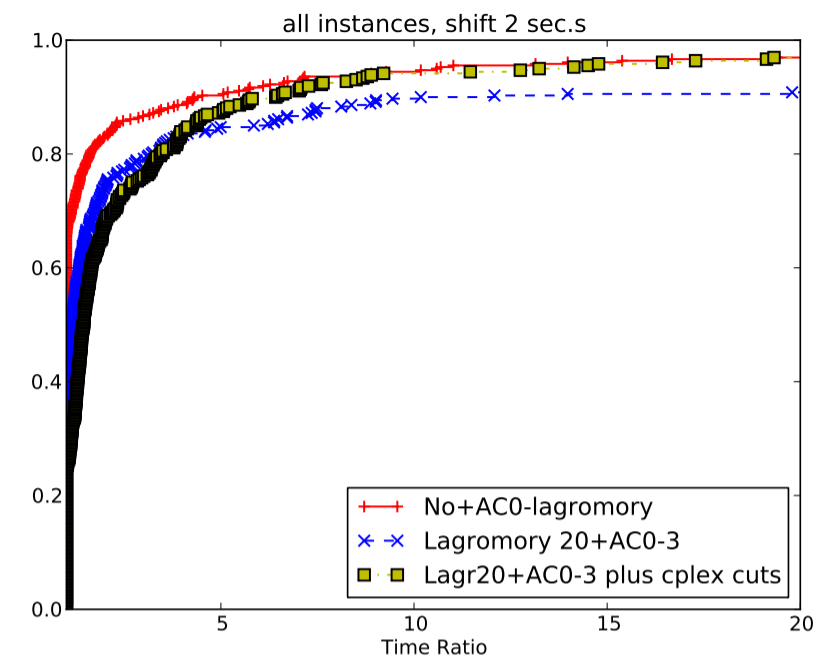
\includegraphics[scale=0.6]{Images/profile_out}\\ 
\end{center} 
\end{figure}
}
\end{itemize}